
\section{Discussion}
\label{section:Discussion:Discussion}


This section presents the underlying discussion creating the basis for the model framework proposed in \Cref{section:Architecture}.
The discussion concerns the current state of time-series prediction, the motivation behind the method selection, model structure, and the selected error metric.
This section intendeds to answer the research questions proposed in this paper,
as well as the reason behind the framework.


%s\import{./sections/Conclusion/Discussion}{CurrentPredictions.tex}
%s\import{./sections/Conclusion/Discussion}{ProposedFramework.tex}
%s\import{./sections/Conclusion/Discussion}{ModelStructure.tex}
% \import{./sections/Conclusion/Discussion}{ErrorMetric.tex}

\subsection{Datasets Characteristics}
The results we get reveals a lot of information about the Characteristics of the different datasets.
The sMAPE is our best indicator for how well the prediction graph fits the target graph.
The 1-day MASE gives us an indicator for how well our predictions are compared to the naive
prediction. It is worth noting that how good the naive prediction is differs from time series
to time series. In a random-walk the naive prediction will be the best possible prediction.
This is also true for time series with a really high autocorrelation coefficient.
The same is true for the 7-day MASE. A time series with a strong weekly seasonality will
give a higher MASE compared to a time series with a low weekly seasonality.
Therefore comparing MASEs from different datasets can be misleading without knowledge of
the underlying characteristics of these series.

Looking at the results we can make some educated guesses of these time series characteristics.
We get the best forecasts fits from dataset 1, which has a mean sMAPE of $0.2034$.
Second comes dataset 3 with a sMAPE of $0.4362$. The hardest dataset to forecast was dataset 2 with a
sMAPE of $0.697$. Looking at the 1-day MASE we can expect the mean autocorrelation coefficient for
dataset 3 to be the highest among the three, with a MASE of $2.009$.
Dataset 1 and 3 should have a high weekly seasonality.

\todo[inline]{Fetch autocorrelation for the different datasets and check our guesses.}

In general, using sMAPE as metric, dataset 2 seems to be the most difficult dataset to forecast.
This makes sense when because the dataset consists of many waslty different time series,
with few obvious pattarns.
\todo[inline]{Write more detail about what kind of time series are in the different datasets in Data
  Section and reference it here}.
% TODO Discussion
% Skrive om forskjellene mellom resultatene mellom datasetene og hva det kan indikere
% dataset 1 sterk ukentli seaason
% dataset 2 svak ukentlig season
% Dataset 2 sterkere årlig season og høyere autocorrelation som gir høyere MASE
% Dataset 3 veldig høy autocorrelation litt dårligere ukentli season
% Kan se ut som SARIMA er bedre enn LSTM til å håndtere årlige sesonger
% Men multivariate LSTM er aller best på årlige sesonger.


\subsection{Modeling seasonality}
Our empirical results indicates that LSTMs have trouble modeling early seasonality.
The dataset with the least yearly seasonality is dataset 1. This is the only dataset where
the univariate LSTM outperformed SARIMA. However when feeding the LSTM with additional
data such as day of the week, month, and season, it became significantly better on datasets
on time series with high yearly seasonality.
\todo[inline]{Finnish experiments with deseasonalisation and write about the result}

These findings contradict \cite[]{Hewamalage2021}.... [TODO: Finnish]



%% Globale metoder gjør det bedre enn locale på MASE, men dårligere på sMAPE
% Kan det være fordi sMAPE straffer under predictions hardere enn 
% over predictions? TODO: Kjøre eksperiment på nytt for å få figures.

\subsection{Global versus Local models}
Comparing the local univariate against the global univariate model across all datasets,
the global model has a sMAPE performance increase of $2.4\%$ on dataset 1, $3.2\%$ on dataset 2 and
$4.9\%$ on dataset 3. This is surprising as the performance increase does not seem to correlate
with the how homogeneous the time series in the dataset are to each other.
Dataset 1, which is the most homogeneous set of them all has the least performance increase.
What might explain these results is that the performance increase is closely connected to the amount
of data available. Dataset 1 consists of the longest time series.
Dataset 3 has the least amount of data
\todo[inline]{Fact check these claims, and add the time series lengths to back up!}
These results support \cite[]{Montero-Manso2021} preposition that global models can give
improve forecasting accuracy, even if the strong assumption that the time series
is generated by the same process.

The same performance increase is not to be found on the multivariate models.
The local multivariate models are really good at capturing the trend and seasonality of
a given product category. This does not seem to translate well to a global model.
One might expect that global models should be able to learn seasonality across
time series if the series contains the same seasonality. But our results show the opposite.
The dataset that suffer the most from making a multivariate local model global is dataset 3
with a sMAPE perfomance loss of $-37\%$. Dataset 1 and dataset 2 got $-10.38\%$ and $-6.47\%$ loss
respectively.
One explanation for this might be that even though all categories in dataset 3 are popular during the
winter, and peaks around the same months, their seasonality is not enough in sync.
For example \textit{"Vintersko"} and \textit{"Vinterjakke"} has their biggest peaks around oktober
when the weather starts becoming cold. While \textit{"Langrennski"} and \textit{"Skisko"}
peaks around january, when the snow starts falling. For a NN which can not differentiate between
which category it is looking at, this will seem like conflicting information which will
hurt the NNs modeling capability.



TODO:
% Write about which dataset the global model performs best on.
%The global models seems to be doing be doing...
%
%Reasons for why global models does not perform better?
%The time series consist of enough data for the local models to generalize
%\cite{Montero-Manso2021}.

% Difference between MASE ans sMAPE
The global models seem to have a better 1 day MASE, but a lower sMAPE.
This is likely because sMAPE is not a symetric metric, as it punishes
under forcasts higher than over forecasts. Looking at the predictions made by
the local and global models, it seems that the global models in general tends to
under-forcast, and the local models has a tendency to over-forecast.

\subsection{LSTM trend and seasonality}
\begin{itemize}
  \item LSTM and ARIAM seem to have trouble with datasets with yearly seasonalities
  \item {LSTM will perform significantly better on these datasets if additional
        a multivariate version is used with additional information about date}
  \item {If date is not available then detrending the dataset using differencing is a good second alternative}
\end{itemize}


\subsection{Normalization versus Standardisation}
Our initial assumption was to use normalization to scale the data between a
fixed range between -1 and 1 because we did not know if the data would follow a Guassian
distribution. After testing both normalization and standardization,
standardization proved to perform significantly better.
The problem with scaling all values between a fixed range is that huge
outliers use up a lot of the range available, which will result in
most of the data having very small differences in values between them.
This can affect the NNs ability to differentiate between the observations.

\Cref{fig:time-series-standardization-vs-normalization} show two different time series
scaled with both techniques
\begin{figure}[h!]
  \centering
  \caption{Effects of different scaling techniques on a dataset with huge outliers.}
  \label{fig:time-series-standardization-vs-normalization}
  \begin{subfigure}[b]{0.49\textwidth}
    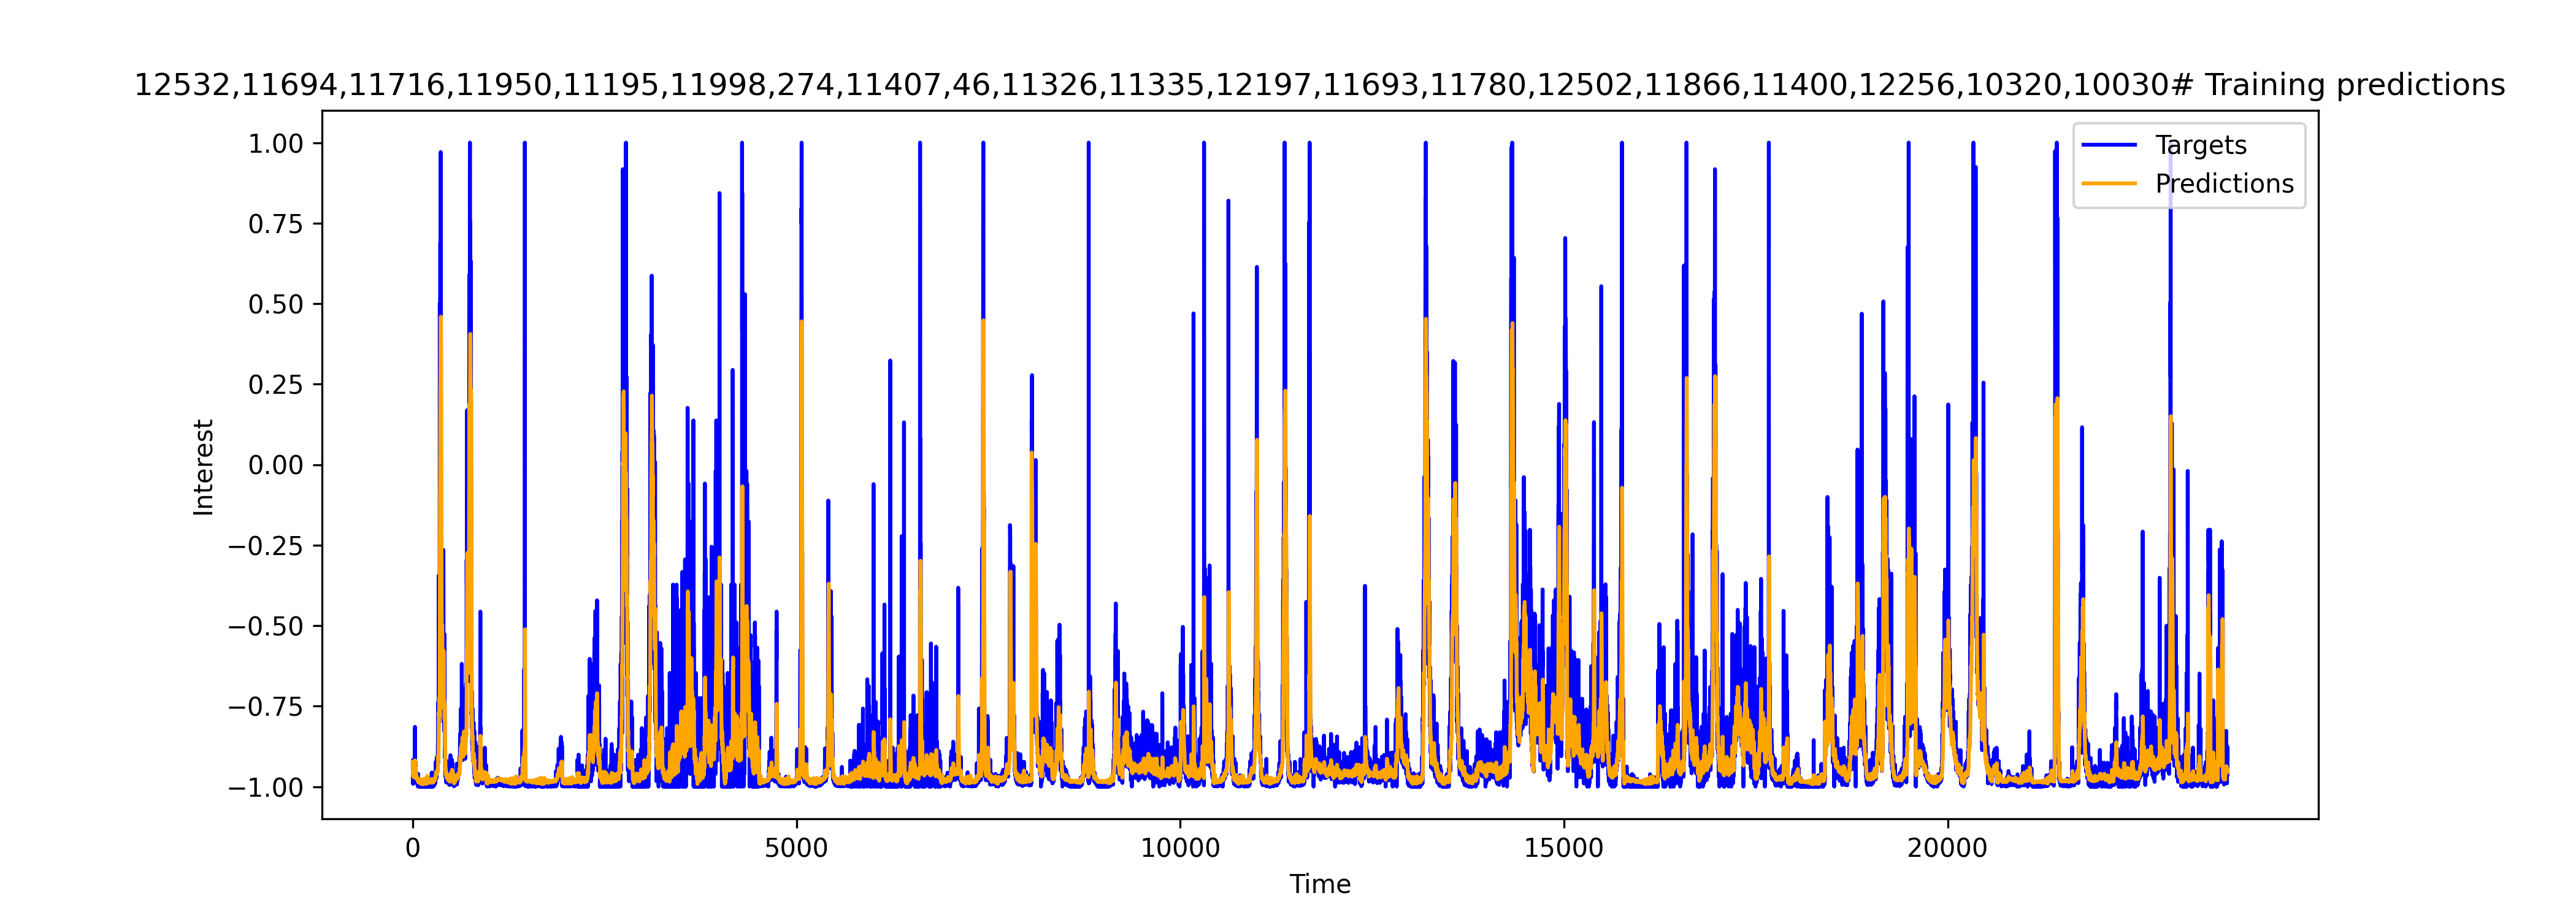
\includegraphics[width=\textwidth]{./figs/dataset/time-series_scaled_normalization2.png}
    \hfill
    \caption{A time series with huge outliers scaled using normalization. Most values are squeezed between -1 and -0.75.}
    \label{fig:time-series-normalization}
  \end{subfigure}
  \begin{subfigure}[b]{0.49\textwidth}
    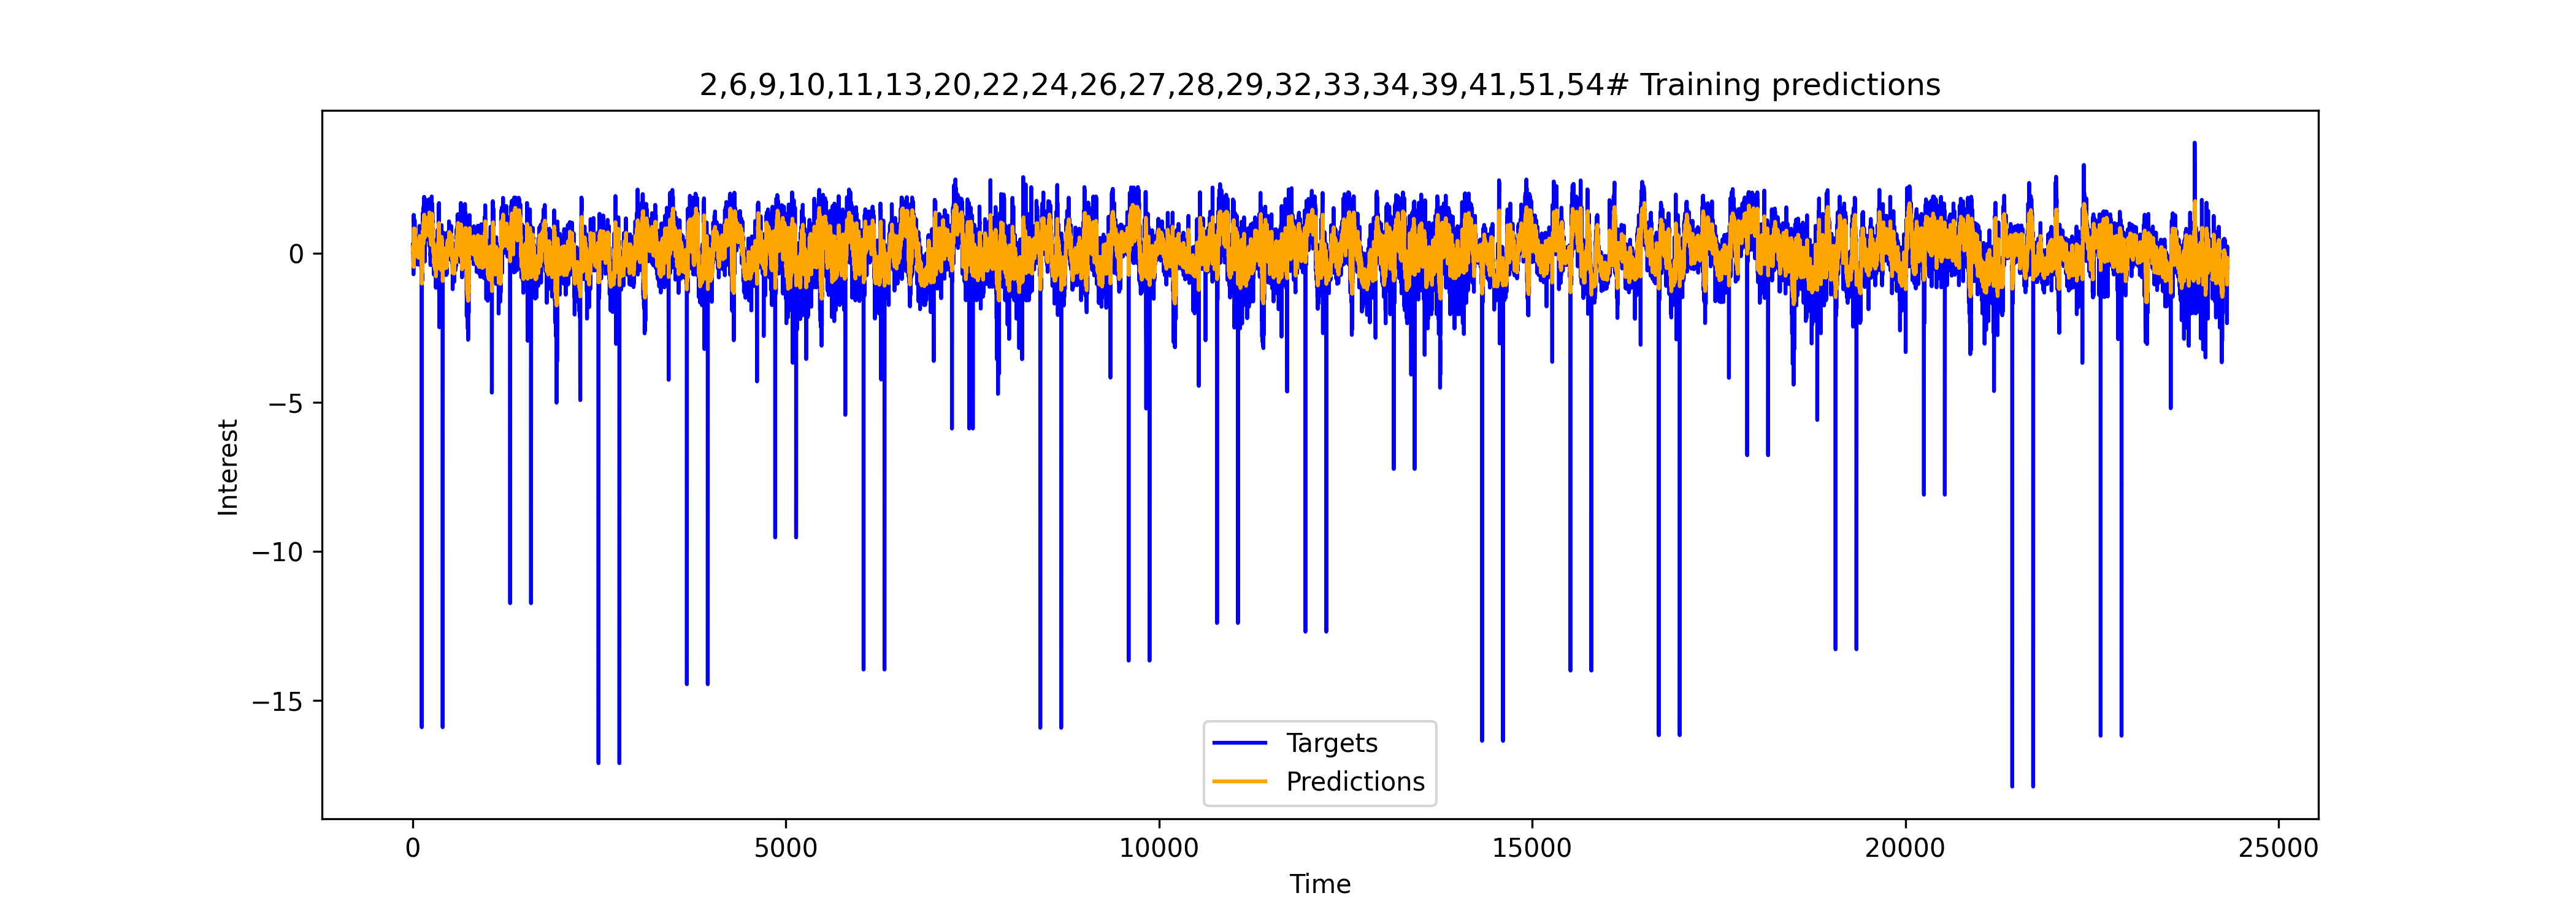
\includegraphics[width=\textwidth]{./figs/dataset/time-series_scaled_standardization.png}
    \hfill
    \caption{A time series scaled using standardization. Most values are centered between -2 and 2.}
    \label{fig:time-series-standardization}
  \end{subfigure}
\end{figure}

\subsection{Which datasets did we get poor results on and why?}
Low mase seems to correlate with a low autocorr.
High smape seem to correlate with early seasonality.

It seems much harder to predict december.
There is a correlation around 0.28 between a categorys MASE metric
and it's autocorrelation coefficient.

\iffalse
  On dataset 2 cat
  Low mase:
  11780
  - low stnd
  - low mase
  - high smape
  - sudden shift in behavior last year
  - some seasonality
  - autocorr 0.78 (pretty low)

  11694
  - few big spikes
  - low mase
  - low smape
  - low seasonality
  - very low autocorr (0.35)
  - consistent smushed lag plot

  1716:
  - low mase
  - high smape
  - low stnd
  -  very high seasonality
  - lots of variation in the dataset
  - consistent "column" in lag plot
  - autotorr 0.86


  11400
  - high mase
  - medium high smape
  - high seasonality
  - not much variation
  - lag plot ok structure like acolumn
  - 0.85 autocorr (predty high)

  11195
  - high mase
  - medium smape
  - early seasonality
  - few big spikes
  - low variation
  - high autocorr

  10320
  - high mase
  - medium smape
  - high autocorr
  - early seasonality

  Data set 10
  - low mase
  - low smape
  - low seasonality
  - low std
  - 0.78 autocorr (low)
  - samlet lag plot

  data set 28
  - high smape
  - low-ish mase
  - low autocorr 0.52
  - low stnd
  - messy lag plot mye spredning
  - some seasonality
  - very noisy

  data set 51
  - low smape
  - high mase
  - samlet lag plot
  - 0.8 autocorr
  - some seasonality

  data set 24
  - high mase
  - low smape
  - 0.83 autocorr
  - small seasonality
  - structure men spredning i scatter plot.
\fi